\chapter{Antenna Fundamentals and Common Designs}
\label{ch:antennas}

An antenna is the transducer between guided energy on a transmission
line and free-space electromagnetic waves (Chapter~\ref{ch:fields}),
working identically (by reciprocity) whether transmitting or receiving.
This chapter covers the core parameters used to describe any antenna,
then surveys the designs an amateur is most likely to build or use.

\section{Radiation: Why an Oscillating Charge Radiates}

An accelerating (including oscillating) electric charge radiates
electromagnetic energy. A current-carrying conductor driven at radio
frequency has continuously accelerating charge carriers, and therefore
radiates --- but efficient radiation requires the conductor's length to
be comparable to the signal's wavelength (Chapter~\ref{ch:fields}, $c =
f\lambda$); a conductor much shorter than a wavelength radiates very
inefficiently, which is why antenna dimensions scale directly with
operating wavelength.

\section{The Half-Wave Dipole}

\bookfig[0.55]{antena_dipolo.png}{A center-fed half-wave dipole antenna.}

The \textbf{half-wave dipole} --- two straight conductors, each
approximately a quarter-wavelength long, fed at the center --- is the
fundamental reference antenna against which most others are compared.
Its resonant length, accounting for the practical fact that RF
propagates slightly slower along a real (finite-diameter) wire than in
free space (the \textbf{velocity factor} or ``end effect''), is
approximately
\[
\boxed{\ell_{\text{ft}} = \frac{468}{f_{\text{MHz}}}} \qquad \text{or equivalently} \qquad
\ell_{\text{m}} \approx \frac{143}{f_{\text{MHz}}}
\]
for total dipole length. (The free-space half-wavelength would be
$\ell = c/(2f) = 150/f_{\text{MHz}}$ metres; the shortening factor,
roughly 0.95, accounts for end effect in typical thin-wire
construction.)

\begin{examplebox}[Dipole length]
Find the total length of a half-wave dipole for 7.100\,MHz.

\emph{Solution.}
\[
\ell_{\text{m}} \approx \frac{143}{7.100} \approx 20.1\,\text{m}.
\]
Each leg is therefore approximately 10.1\,m.
\end{examplebox}

A resonant half-wave dipole in free space presents a feedpoint
impedance of approximately $73\,\Omega$ (resistive, at resonance),
reasonably close to standard 50\,$\Omega$ coax, though height above
ground and surroundings shift this value somewhat in practice. A dipole
fed at its center is inherently a \textbf{balanced} load and should be
fed through a balun (Chapter~\ref{ch:transformers}) if connected to
unbalanced coaxial cable, to avoid feedline radiation and pattern
distortion.

\section{Radiation Pattern, Gain, and Directivity}

An antenna's \textbf{radiation pattern} describes how strongly it
radiates as a function of direction. Even the simplest dipole is not
omnidirectional in three dimensions: it radiates a figure-eight pattern
broadside to the wire (maximum) and radiates essentially nothing off the
ends of the wire (nulls).

\textbf{Directivity} and \textbf{gain} quantify how much an antenna
concentrates radiation in its favored direction(s) compared to a
reference. Gain, expressed in \textbf{dBi} (relative to a theoretical
isotropic radiator) or \textbf{dBd} (relative to a reference dipole),
was defined precisely in Chapter~\ref{ch:decibels}; a real dipole has
about 2.15\,dBi (0\,dBd) of gain in its favored broadside directions,
simply from concentrating energy away from the (nulled) end directions
rather than spreading it equally in all directions like a true
isotropic source.

\begin{keyidea}[Gain is a trade, not free energy]
An antenna cannot amplify signal power --- gain in one direction is
always achieved by concentrating radiation that would otherwise have
gone elsewhere, not by adding energy. A high-gain directional antenna
therefore radiates \emph{less} in directions away from its main lobe
than an isotropic radiator would, even as it radiates significantly
\emph{more} in its favored direction.
\end{keyidea}

\section{Antenna Efficiency and Losses}

\bookfig[0.55]{antena_eficiencia.png}{Antenna efficiency: radiated
power vs.\ power lost to resistive and ground losses.}

Real antennas dissipate some power as heat rather than radiating it all,
due to conductor resistance, loading-coil losses, and losses in nearby
lossy ground or objects. \textbf{Radiation efficiency} is
\[
\eta = \frac{R_{\text{rad}}}{R_{\text{rad}}+R_{\text{loss}}} \times 100\%
\]
where $R_{\text{rad}}$ is the antenna's \textbf{radiation resistance}
(the equivalent resistance that would dissipate the same power as is
actually radiated) and $R_{\text{loss}}$ lumps together all real
resistive losses. Electrically short antennas (loaded verticals and
mobile whips well under a quarter-wavelength, for instance) tend to have
low radiation resistance, making loss resistance a proportionally larger
fraction of the total and efficiency correspondingly poorer --- a key
reason full-size or close-to-full-size antennas generally outperform
heavily shortened/loaded designs when space permits.

\section{Polarization and Ground Effects}

An antenna's orientation sets its \textbf{polarization}
(Chapter~\ref{ch:fields}): a horizontal dipole radiates
horizontally polarized waves; a vertical antenna radiates vertically
polarized waves. Ground reflections interact strongly with a nearby
antenna, modifying both its feedpoint impedance and its radiation
pattern (particularly the low-angle performance important for
long-distance HF propagation, Chapter~\ref{ch:propagation}); antenna
height above ground, in wavelengths, is therefore a major practical
design variable, not just an installation convenience.

\section{The Yagi--Uda Antenna}

\bookfig[0.6]{antena_yagi.png}{A Yagi--Uda beam antenna: driven
element, reflector, and directors.}

The \textbf{Yagi--Uda} antenna (commonly just ``Yagi''), invented by
Shintaro Uda and popularized by Hidetsugu Yagi in the 1920s, achieves
significant directional gain from a single driven half-wave dipole
element by adding nearby \textbf{parasitic elements}: a slightly longer
\textbf{reflector} behind the driven element and one or more slightly
shorter \textbf{directors} in front of it. These parasitic elements are
not directly fed; they are excited by mutual coupling with the driven
element's near field, and their carefully tuned length and spacing
cause constructive interference in the forward direction and
destructive interference to the rear, producing a directional beam
pattern with useful gain (typically 6--15\,dBi depending on the number
of elements and boom length) and a front-to-back ratio that helps reject
interference and noise arriving from behind the antenna.

\section{Ground-Plane and Vertical Antennas}

\bookfig[0.5]{antena_ground_plane.png}{A quarter-wave ground-plane
vertical antenna with radial elements.}

A \textbf{ground-plane vertical} uses a quarter-wave vertical radiator
fed against a set of radial elements (or an actual conductive ground
plane) that serve as the antenna's ``other half,'' effectively forming
half of a dipole with an electrical mirror image below the
feedpoint. Feedpoint impedance for an ideal quarter-wave vertical over a
perfect ground plane is approximately $36\,\Omega$ (roughly half the
dipole's $73\,\Omega$, consistent with the mirror-image picture).
Verticals radiate omnidirectionally in azimuth (all compass directions
equally) with vertical polarization, and --- with a low radiation angle
particularly useful for DX contacts --- are popular where a horizontal
antenna large enough for the operating band is impractical, at the cost
of typically needing an effective radial/ground system to perform well.

\section{Loop Antennas}

\bookfig[0.5]{antena_loop_magnetica.jpg}{A small transmitting magnetic
loop antenna.}

A \textbf{loop antenna} forms a closed (or nearly closed) conductive
loop. \textbf{Full-size loops} (a wavelength or more in circumference)
behave broadly like a folded dipole variant with useful gain and
different polarization/pattern characteristics depending on
orientation. \textbf{Small (magnetic) loops}, with circumference well
under a wavelength, are physically compact and couple predominantly to
the magnetic near-field component; they achieve resonance using a
high-voltage tuning capacitor across the loop and, despite modest
radiation efficiency for their small size, are valued for
space-constrained installations and for a naturally narrow bandwidth
that provides useful front-end selectivity even before a receiver's own
filtering.

\section{Multiband and Wire Antenna Techniques}

\begin{figure}[H]
\centering
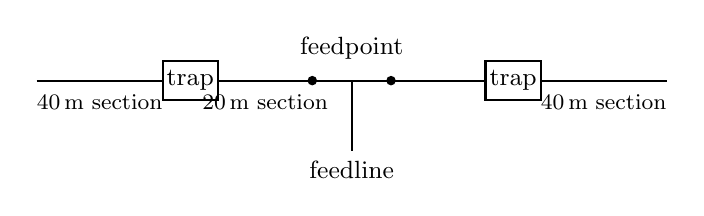
\begin{tikzpicture}[scale=1,every node/.style={font=\small}]
\draw[thick] (0,0) -- (1.6,0);
\draw[thick] (1.6,-0.25) rectangle (2.3,0.25) node[midway]{trap};
\draw[thick] (2.3,0) -- (3.5,0);
\filldraw (3.5,0) circle (1.5pt);
\draw[thick] (3.5,0) -- (4.5,0);
\filldraw (4.5,0) circle (1.5pt);
\draw[thick] (4.5,0) -- (5.7,0);
\draw[thick] (5.7,-0.25) rectangle (6.4,0.25) node[midway]{trap};
\draw[thick] (6.4,0) -- (8,0);
\draw[thick] (4,0) -- (4,-0.9);
\node[below] at (4,-0.9) {feedline};
\node[below,align=center] at (0.8,-0.05) {\footnotesize 40\,m section};
\node[below,align=center] at (2.9,-0.05) {\footnotesize 20\,m section};
\node[below,align=center] at (7.2,-0.05) {\footnotesize 40\,m section};
\node[above] at (4,0.15) {feedpoint};
\end{tikzpicture}
\caption{A trap dipole: LC traps present a high impedance at their
design frequency, electrically shortening the antenna so a single wire
resonates on more than one band.}
\end{figure}

\begin{itemize}
\item \textbf{Trap dipoles/verticals}: parallel LC resonant circuits
(\textbf{traps}, Chapter~\ref{ch:rlc-resonance}) inserted along the
antenna element present a high impedance (effectively an open circuit,
electrically shortening the antenna) at their design frequency, letting
a single physical antenna present resonant electrical lengths on
several different bands.
\item \textbf{End-fed half-wave (EFHW) antennas}: a half-wave wire fed
at (or very near) one end, where feedpoint impedance is very high
(thousands of ohms) rather than the ${\sim}73\,\Omega$ of a center-fed
dipole; a purpose-built impedance-matching transformer converts this
high impedance down to $50\,\Omega$, letting the antenna be fed
conveniently from one end rather than requiring center support.
\item \textbf{Folded dipoles}: a dipole with a second parallel
conductor connecting its two ends, raising feedpoint impedance
(approximately $4\times$ a plain dipole's, or about $280$--$300\,\Omega$
for a simple two-wire fold) and providing a somewhat broader bandwidth
--- the classic feed for 300\,$\Omega$ balanced television ribbon line
and folded-element Yagi driven elements.
\end{itemize}

\begin{figure}[H]
\centering
\begin{tikzpicture}[scale=1,every node/.style={font=\small}]
\draw[thick] (0,0) -- (6.4,2.1);
\node[above] at (3.2,1.05) {half-wave wire ($\approx\lambda/2$)};
\draw[thick] (6.4,2.1) circle (2.5pt);
\node[above right] at (6.4,2.1) {end support/insulator};
\draw[thick] (-0.3,-0.4) rectangle (0.5,0.2);
\node[left] at (-0.35,-0.1) {matching transformer};
\draw[thick] (0.1,-0.4) -- (0.1,-1.1);
\node[below] at (0.1,-1.1) {\small 50\,$\Omega$ coax to radio};
\end{tikzpicture}
\caption{An end-fed half-wave (EFHW) antenna. A step-up impedance
transformer (typically 49:1 or 64:1) matches the wire's high end-feed
impedance down to 50\,$\Omega$.}
\end{figure}

\section{Antenna Bandwidth}

\bookfig[0.65]{antena_bandas.png}{Typical amateur HF antenna bandwidth
across several bands.}

An antenna's usable \textbf{bandwidth} (the frequency range over which
its feedpoint impedance stays reasonably close to the feedline's
characteristic impedance, typically judged by SWR) depends on the
antenna's own effective $Q$ (Chapter~\ref{ch:rlc-resonance}): thicker
conductors and lower operating $Q$ generally give wider bandwidth,
which is why a fan dipole, thick aluminum Yagi element, or cage dipole
often covers more of a band comfortably than a thin, single wire of the
same nominal design.

\begin{quickreview}
\item An antenna radiates because it carries oscillating (accelerating)
charge; efficient radiation needs dimensions comparable to a wavelength.
\item Half-wave dipole length (m) $\approx 143/f_{\text{MHz}}$;
free-space feedpoint impedance $\approx 73\,\Omega$.
\item Gain (dBi/dBd) describes concentration of radiation in a favored
direction, not added total power; efficiency $\eta =
R_{\text{rad}}/(R_{\text{rad}}+R_{\text{loss}})$.
\item Yagi--Uda antennas use parasitic reflector/director elements
around one driven element to achieve directional gain.
\item Verticals/ground-planes give omnidirectional, low-angle,
vertically polarized radiation; loops, traps, EFHW, and folded-dipole
techniques address space, multiband, and feed-impedance needs.
\end{quickreview}

\begin{practiceproblems}
\item Find the total length of a half-wave dipole for 21.200\,MHz.
\item A Yagi has 10\,dBi of gain. Express this in dBd.
\item Explain why an electrically short, heavily loaded mobile whip
antenna typically has lower efficiency than a full-size dipole on the
same band.
\item Explain, in terms of the mirror-image picture, why a quarter-wave
ground-plane vertical's feedpoint impedance is roughly half that of a
half-wave dipole.
\item Explain the practical purpose of a matching transformer on an
end-fed half-wave antenna, given that a half-wave wire's end-fed
impedance is very high rather than close to 50\,$\Omega$.
\end{practiceproblems}
